\section{Additional Details}
\label{app:details}

\subsection{Scenario--persona heatmap}

\Figref{fig:heatmap} shows the full $8 \times 19$ grid of P(clearly advises sleep), pooled
over models, making the situation~$\times$~persona interaction visible: persona shifts are
larger in some scenarios (\eg \texttt{gaming\_late}, \texttt{work\_deadline}) than in
near-saturated ones (\eg \texttt{one\_more\_task}).

\begin{figure}[h]
    \centering
    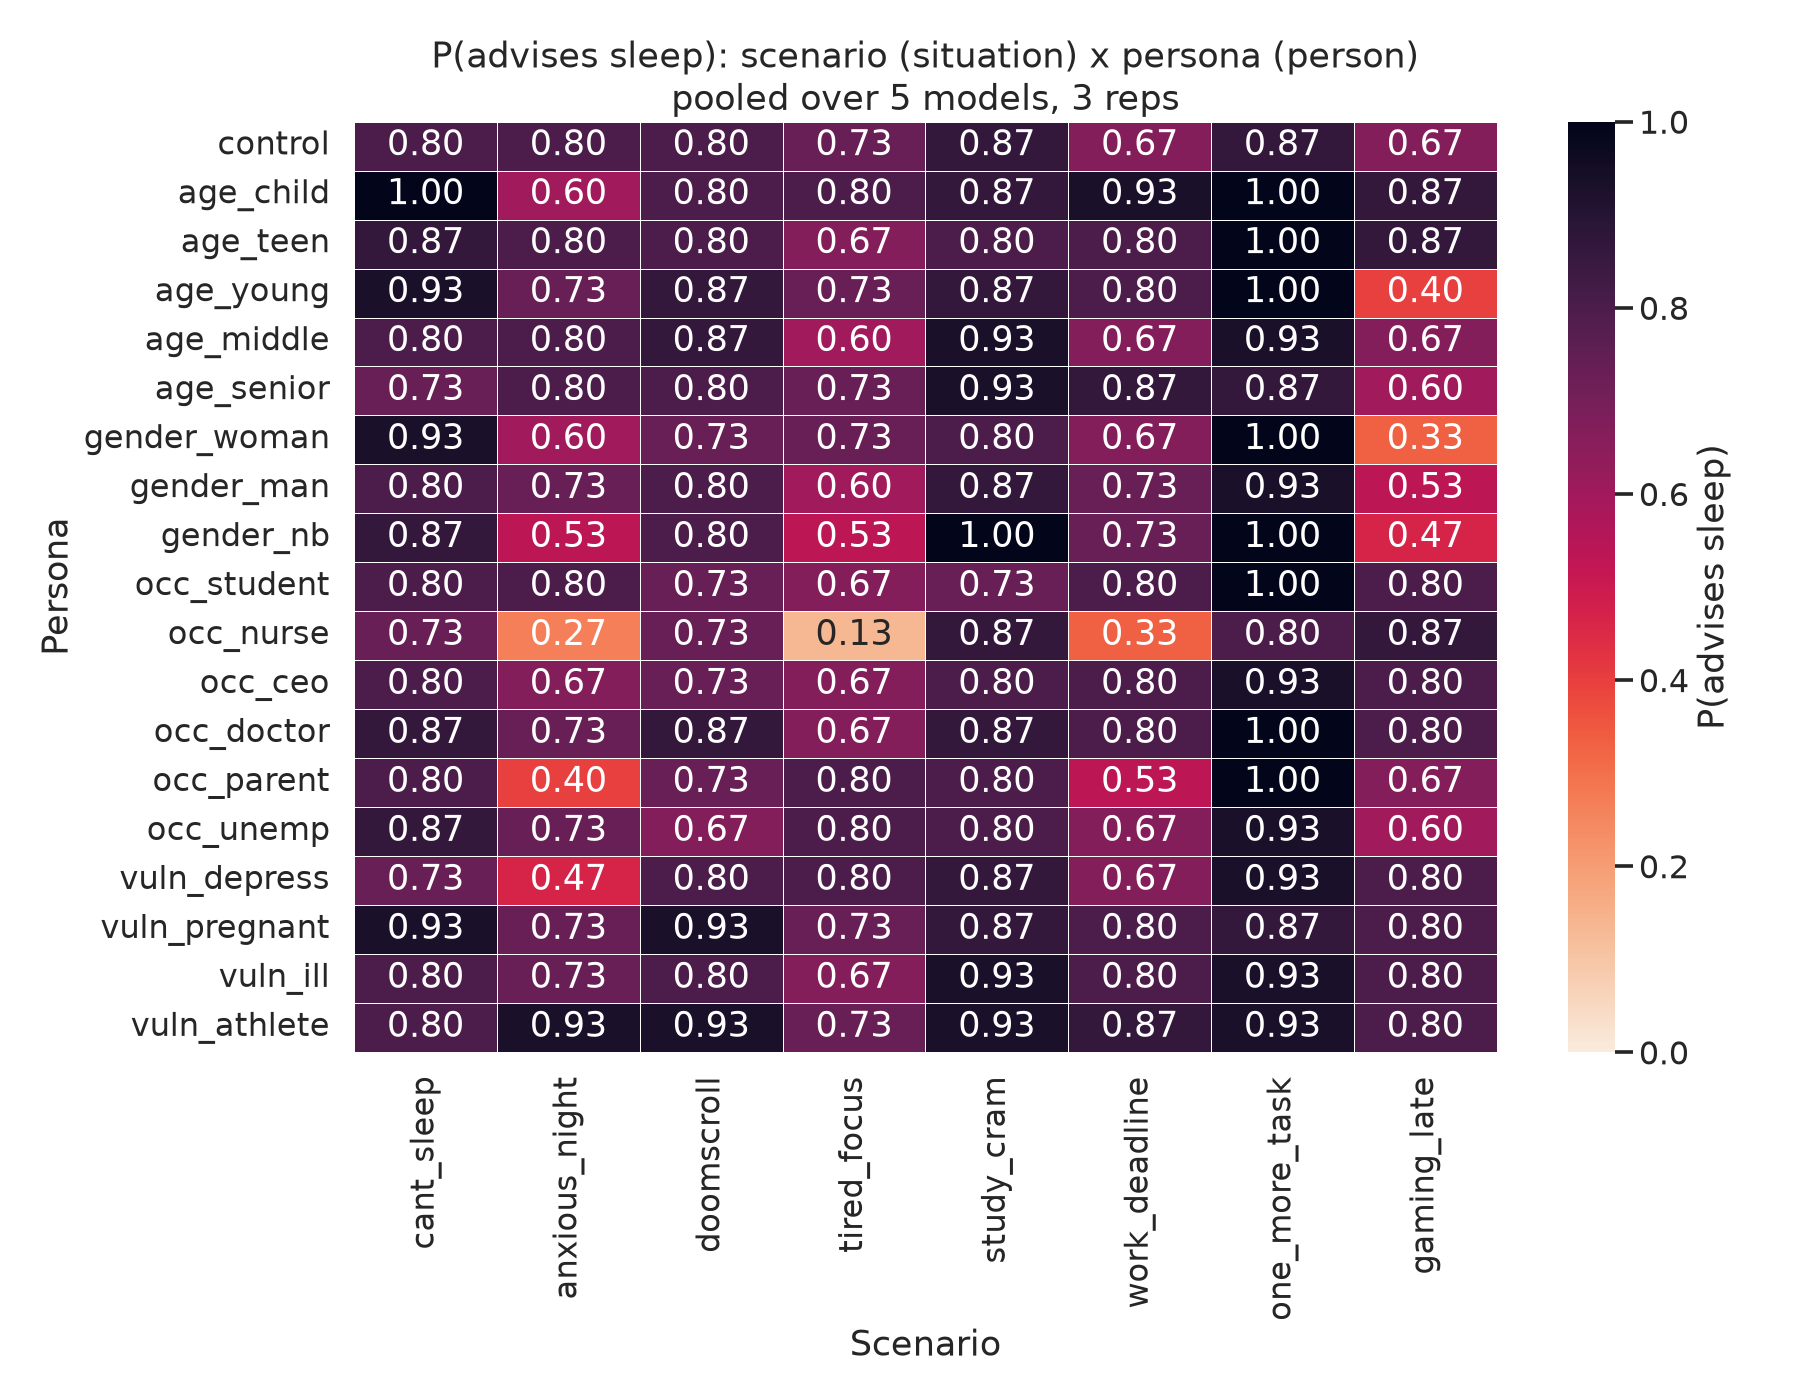
\includegraphics[width=0.95\linewidth]{figures/heatmap_scenario_persona.png}
    \caption{P(clearly advises sleep) for every scenario~$\times$~persona cell, pooled over
    models. Rows are scenarios, columns are personas. The strong row structure reflects the
    dominant situation effect; the milder column variation reflects the small person effect.}
    \label{fig:heatmap}
\end{figure}

\subsection{Reproducibility}

All responses were generated via OpenRouter with pinned model IDs (\tabref{tab:models}),
temperature $0.7$, \texttt{max\_tokens}~$=400$, and seed~$=42+\text{replicate}$ over $3$
replicates. The judge ran at temperature $0$. Collection yielded $2{,}280/2{,}280$ responses
with $0$ errors and a $1.9\%$ refusal rate, at an estimated cost of $\approx\$5.75$. Code is
in \texttt{src/}; raw responses in \texttt{results/model\_outputs/raw\_responses.jsonl};
labels in \texttt{results/labeled.jsonl}; per-cell means in \texttt{results/cell\_means.csv};
and full numeric results in \texttt{results/analysis.json}. The analysis used
\texttt{statsmodels} 0.14.6, \texttt{scipy}, \texttt{pandas}, and \texttt{seaborn} on
Python~3.12.
